\documentclass{article}
\usepackage[utf8]{inputenc}
\usepackage[english]{babel}
\usepackage{graphicx}
\usepackage{subfiles}
\usepackage{fancyhdr}
\usepackage{nameref}
\usepackage{hyperref}
\usepackage{mathabx}
%\usepackage{gensymb}

\usepackage[left=10mm,right=30mm,top=25mm,bottom=25mm]{geometry}

\graphicspath{{images/}{../images/}}
 
\title{Naturwissenschaften Skriptum}
\author{Simon Lehner-Dittenberger}
\date{ \today }
\makeindex
 
\pagestyle{fancy} 
\fancyhf{} %alle Kopf- und Fußzeilenfelder bereinigen
\rhead{Simon Lehner-D.}
\chead{\leftmark}
\lhead{\today} 
\rfoot{Seite \thepage}

\setlength{\parindent}{0pt}
\setlength{\parskip}{\baselineskip}

\begin{document}

\maketitle
\begin{figure}[bh]
\centering
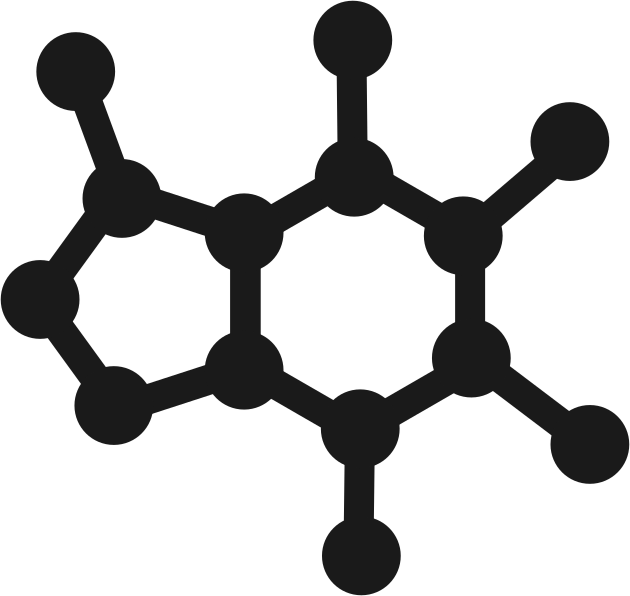
\includegraphics[width=4cm]{caffeine.png}
\end{figure}
\newpage

\tableofcontents 
\newpage

 
\section{Einleitung}
\subfile{sections/introduction}
\newpage
 
\section{Klassische Physik}
\subfile{sections/klassische_physik}
\newpage

\section{Schwingungen und Wellenphänomene}
\subfile{sections/schwingungen_und_wellen}
\newpage

\section{Moderne Physik}
\subfile{sections/moderne_physik}
\newpage

\section{Anorganische Chemie}
\subfile{sections/anorganische_chemie}
\newpage

\section{Biotechnologie}
\subfile{sections/biotechnologie}
\newpage

\section{Umwelt und Gesellschaft}
\subfile{sections/umwelt_und_gesellschaft} 
\newpage
 
\end{document}